\label{sec:problema}

\subsection{O DUNE, o FD3 e a luz de cintilação}
\label{sec:detector}

O DUNE (\textit{Deep Underground Neutrino Experiment}) estudará a oscilação de neutrinos com um feixe do Fermilab e um detector distante a \qty{1300}{\km}; seus objetivos incluem a violação de CP (conjugação de carga e paridade), o ordenamento das massas, os neutrinos de supernovas e o decaimento do próton \cite{abi2020volume}. Conforme \citeonline{abud2024dunephase}, o detector distante usa câmaras de projeção temporal de argônio líquido (LArTPCs); a Fase~II acrescenta o terceiro módulo (FD3), de deriva vertical como o segundo (FD2), e o sistema de detecção de fótons do FD3 será definido pelo programa APEX (\textit{Aluminum Profiles with Embedded X-ARAPUCA}).

Partículas carregadas ionizam e excitam o argônio: os elétrons derivam até os planos de leitura, que dão as coordenadas perpendiculares à deriva, e a cintilação (cerca de \num{24000} fótons por MeV a \qty{500}{\V\per\cm}, perto de \qty{127}{\nm}) marca o instante $t_0$ da interação, do qual depende a coordenada de deriva \cite{abi2020volume}. Neutrinos de supernovas têm energias da ordem de \qty{10}{\MeV} \cite{abi2021supernova}; nesse regime, a posição obtida da luz ajuda a selecionar o volume fiducial e a rejeitar fundos radiológicos \cite{paulucci2022dune}. Abaixo de \qty{5}{\MeV}, o papel da luz em depósitos isolados é pouco explorado \cite{caratelli2022low}.

O APEX prevê nos perfis da gaiola de campo cerca de \num{7000} fotodetectores X-ARAPUCA de \qtyproduct{50 x 50}{\cm}, com cobertura óptica próxima de \qty{60}{\percent} \cite{marinho2025apex}; cada um desloca o comprimento de onda da luz e a aprisiona até ser detectada por fotomultiplicadores de silício \cite{machado2018xarapuca}. Simulado com eficiência de detecção de \qty{2}{\percent}, o APEX tem, na região central, rendimento luminoso (LY) de \num{180} fotoelétrons (p.e.)\ por MeV em média e \qty{109}{\pe\per\MeV} no mínimo, e LY maior nas extremidades; estimadores analíticos reconstroem posição e energia \cite{marinho2025apex}.

\subsection{Dados simulados e regime de contagem de fótons}
\label{sec:dados}

A simulação é a da etapa anterior \cite{vicentin2024study}: \num{9364} eventos com energia depositada $E = {}$\qty{100}{\MeV}. O vértice $\mathbf{v} = (x, y, z)$ está no referencial dos sensores, usado em todo o relatório; no referencial dos nomes de arquivo (Seção~\ref{sec:dados_grafos}), ele é $\mathbf{t} = (t_x, t_y, t_z)$, e \mbox{$(x, y, z) = (t_y, -t_x, t_z)$}. Os vértices formam uma grade de \numproduct{13 x 12 x 60}~$=$~\num{9360} posições espaçadas de \qty{0.5}{\m} (\qty{0.45}{\m} no primeiro passo em $x$), num octante: $x$ de \num{0.05} a \qty{6.0}{\m}, $y$ de \num{-5.5} a \qty{0}{\m} e $z$ de \num{0} a \qty{29.5}{\m}. Quatro delas têm dois eventos. Há \num{6912} canais, de posições $\mathbf{p}_i$: \num{2880} em cada parede longa ($y = {}$\qty{\pm 6.673}{\m}), \num{576} em cada tampa ($z = {}$\qty{\pm 29.93}{\m}) e nenhum nas faces normais a $x$; esse total é o de uma gaiola de campo do APEX totalmente instrumentada, \num{192} módulos de \num{36} fotodetectores \cite{abud2024dunephase}. O eixo longo, $z$, segue o feixe.

Um depósito de \qty{10}{\MeV} é representado por
\begin{equation}
  \tilde{N}_i = \operatorname{round}(s N_i), \qquad n_i \sim \operatorname{Binomial}(\tilde{N}_i, \varepsilon),
  \label{eq:luz}
\end{equation}
em que $N_i$ é o número de fótons que chegam ao canal $i$ na simulação de \qty{100}{\MeV}, já corrigido (Seção~\ref{sec:dados_grafos}); $s = {}$\num{0.1}, o fator de escala; $\tilde{N}_i$, a contagem escalada e arredondada; $\varepsilon = {}$\num{0.02}, a eficiência de detecção suposta pelo APEX \cite{marinho2025apex}; e $n_i$, os fotoelétrons detectados. Cada evento tem um sorteio de fótons (semente \num{42} mais seu índice), comum às épocas e aos modelos.

Os eventos de teste têm em média \qty{530.1}{\pe} (\qty{53.0}{\pe\per\MeV}) em \num{245} canais. Nos \num{9364} eventos, em média só \qty{3.6}{\percent} dos canais registram luz (Figura~\ref{fig:evento_exemplo}); a luz por evento varia de \num{43} a \qty{2334}{\pe} e cai com a distância do vértice à parede longa mais próxima (Figura~\ref{fig:luz_distancia}); no total, essa parede recebe \qty{70.2}{\percent} dos fotoelétrons, a tampa mais próxima, \qty{20.7}{\percent}, e a parede oposta, \qty{9.2}{\percent}. Com o rendimento médio do APEX, um depósito de \qty{10}{\MeV} daria \qty{1800}{\pe}, \num{3.4} vezes a luz média do teste, que equivale a \qty{2.9}{\MeV}, energia da comparação em luz detectada igual (Seção~\ref{sec:protocolo_comparacao}).

\begin{figure}[H]
  \centering
  \begin{subfigure}[t]{0.485\textwidth}
    \centering
    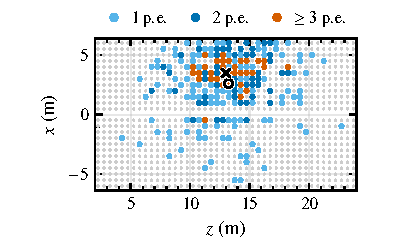
\includegraphics{figures/evento_exemplo.pdf}
    \caption{Parede longa em $y = {}$\qty{-6.673}{\m}, a mais próxima do vértice, no evento de teste \num{5834} (\qty{387}{\pe} em \num{247} dos \num{6912} canais); ela recebe a maior parte da luz, e todos os seus canais com luz estão no trecho exibido. Pontos cinza: canais sem luz; cor: fotoelétrons por canal; cruz: projeção do vértice; círculo: projeção do centroide da luz, onde fica o nó global do grafo (Seção~\ref{sec:dados_grafos}).}
    \label{fig:evento_exemplo}
  \end{subfigure}\hfill
  \begin{subfigure}[t]{0.485\textwidth}
    \centering
    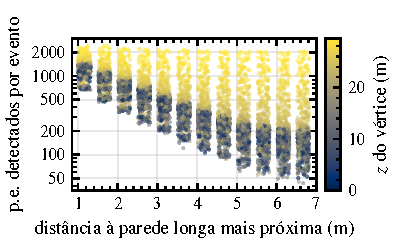
\includegraphics{figures/luz_distancia.pdf}
    \caption{Luz detectada por evento, em escala logarítmica, nos \num{9364} eventos simulados, em função da distância do vértice à parede longa mais próxima; a cor indica a coordenada $z$ do vértice. A luz cai com a distância e é maior perto da tampa. Os vértices ocupam \num{12} distâncias, a cada \qty{0.5}{\m}; os pontos foram deslocados ao acaso na horizontal para reduzir a sobreposição.}
    \label{fig:luz_distancia}
  \end{subfigure}
  \caption{Regime de contagem de fótons: (a) um evento de teste; (b) a luz de todos os eventos simulados.}
  \label{fig:regime_fotons}
\end{figure}

\subsection{Objetivo e formulação da tarefa}
\label{sec:tarefa}

Na etapa anterior \cite{vicentin2024study}, uma rede densa de \num{8195} parâmetros sobre \num{60} descritores selecionados em fases obteve erro absoluto médio (MAE) de teste de \num{12.03} a \qty{18.18}{\cm} por eixo; como os descritores resumem a leitura do detector inteiro, o modelo só recebe o que eles retêm do padrão da luz nos canais. Esta etapa representa cada evento como um grafo dos canais com luz, estima o vértice por passagem de mensagens e compara, nos mesmos eventos de teste, \num{11} codificadores com totais de parâmetros quase iguais (capacidade equiparada), \textit{boosters} ajustados (conjuntos de árvores de decisão: XGBoost e LightGBM) e o baricentro da luz, com os valores citados da rede anterior e o APEX em luz detectada igual. Procura-se ainda onde o erro se concentra e o que o limita.

A tarefa é estimar $\mathbf{v}$ com as posições $\mathbf{p}_i$ e a luz $n_i$ dos canais ativos ($n_i$ não nulo), que formam o conjunto $A$, de $|A|$ elementos.

Para o vértice previsto $\hat{\mathbf{v}}$ e $J$ eventos (\num{937} no teste), calculam-se
\begin{equation}
  \begin{aligned}
    \mathrm{MAE}_a &= \bigl\langle \lvert \hat{v}_a - v_a \rvert \bigr\rangle, &\qquad
    \mathrm{RMSE}_a &= \sqrt{\bigl\langle (\hat{v}_a - v_a)^2 \bigr\rangle}, \\
    \mathrm{RMSE}_{\mathrm{comb}} &= \sqrt{\tfrac{1}{3} \textstyle\sum_{a} \mathrm{RMSE}_a^2}, &\qquad
    \bar{d} &= \bigl\langle \lVert \hat{\mathbf{v}} - \mathbf{v} \rVert \bigr\rangle,
  \end{aligned}
  \label{eq:metricas}
\end{equation}
em que $\langle\cdot\rangle$ é a média sobre os $J$ eventos, $v_a$ e $\hat{v}_a$ são as componentes de $\mathbf{v}$ e $\hat{\mathbf{v}}$ no eixo $a \in \{x, y, z\}$, $\mathrm{MAE}_a$ e $\mathrm{RMSE}_a$ são o MAE e a raiz do erro quadrático médio (RMSE) nesse eixo, $\mathrm{RMSE}_{\mathrm{comb}}$ é o RMSE combinado, que não depende da atribuição dos eixos, e $\bar{d}$ é o erro tridimensional (3-D) médio. O MAE médio é a média dos três $\mathrm{MAE}_a$; $\bar{d}$ é também a perda do treinamento e o critério de ordenação dos codificadores.
